% d6.tex

\documentclass[tikz]{standalone}

\begin{document}
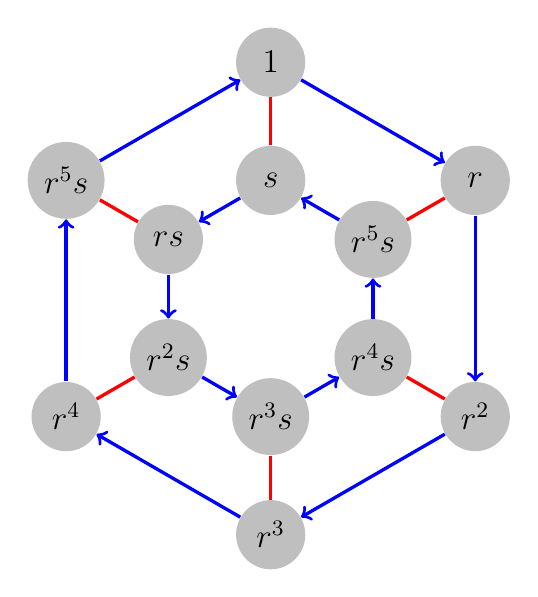
\begin{tikzpicture}[ele/.style = {circle, minimum size = 25pt, fill = lightgray, font = \large},
  s/.style = {-, red, very thick},
  r/.style = {->, blue, very thick},
  rr/.style = {<-, blue, very thick}]
  % inner
  \foreach \angle/\label [count = \name from 0] in {90/s, 30/r^5s, -30/r^4s, -90/r^3s, -150/r^2s, -210/rs} {
	\node (in-\name) [ele] at (\angle:1.5) {$\label$};
  }

  % outer
  \foreach \angle/\label [count = \name from 0] in {90/1, 30/r, -30/r^2, -90/r^3, -150/r^4, -210/r^5s} {
	\node (out-\name) [ele] at (\angle:3.0) {$\label$};
  }

  \foreach \i in {0, 1, ..., 4} {
	\def\next{\the\numexpr\i+1}
	\draw[r] (out-\i) to (out-\next);
	\draw[rr] (in-\i) to (in-\next);

	\draw[s] (in-\i) to (out-\i);
  }
  \draw[r] (out-5) to (out-0);
  \draw[rr] (in-5) to (in-0);
  \draw[s] (in-5) to (out-5);
\end{tikzpicture}
\end{document}
